\chapter{Introduction}
    In this project we wanted to generate visualizations of music tracks with the help of generative adverserial networks (GAN). Our goal was for the visualizations to visibly correlate to the music when played alongside.
    For this we extract different sets of features from the music and use these features as seeds for the generators of our GANs, which we train on sets of real world images, flowers for the most part.

    For the feature extraction, we mainly tried out three different approaches. First, we generated mel spectrograms from the music and used these directly as input. As our second approach, we reduced the size of the mel spectrograms with an autoencoder to then use the encoded vectors as input, and the last approach was to use the featuremap of an intermediate layer of a convolutional recurrent neural network (CRNN), trained to classify the genre of a given song from its corresponding mel spectrogram.

    For our GANs, we had two main architectures which we tried out during the project: deep convolutional generative adverserial networks (DCGAN) and InfoGANs, the latter is an extension of GANs with the addition of maximizing mutual information between a subset of the latent input vector and the observation.

    For the training of the various networks we used the small Free Music Archive~\cite{FMA} dataset as our main source of music with an even distribution of 8000 songs over 8 genres, and the \textit{102 Category Flower}~\cite{102flower} dataset as our main source of real images for the GANs. In the following sections we will explain our different approaches in detail and discuss their varying performance. We will start with the feature extraction, before we go into detail about our GANs until we finally talk about the results.

    \begin{figure}
        \centering
        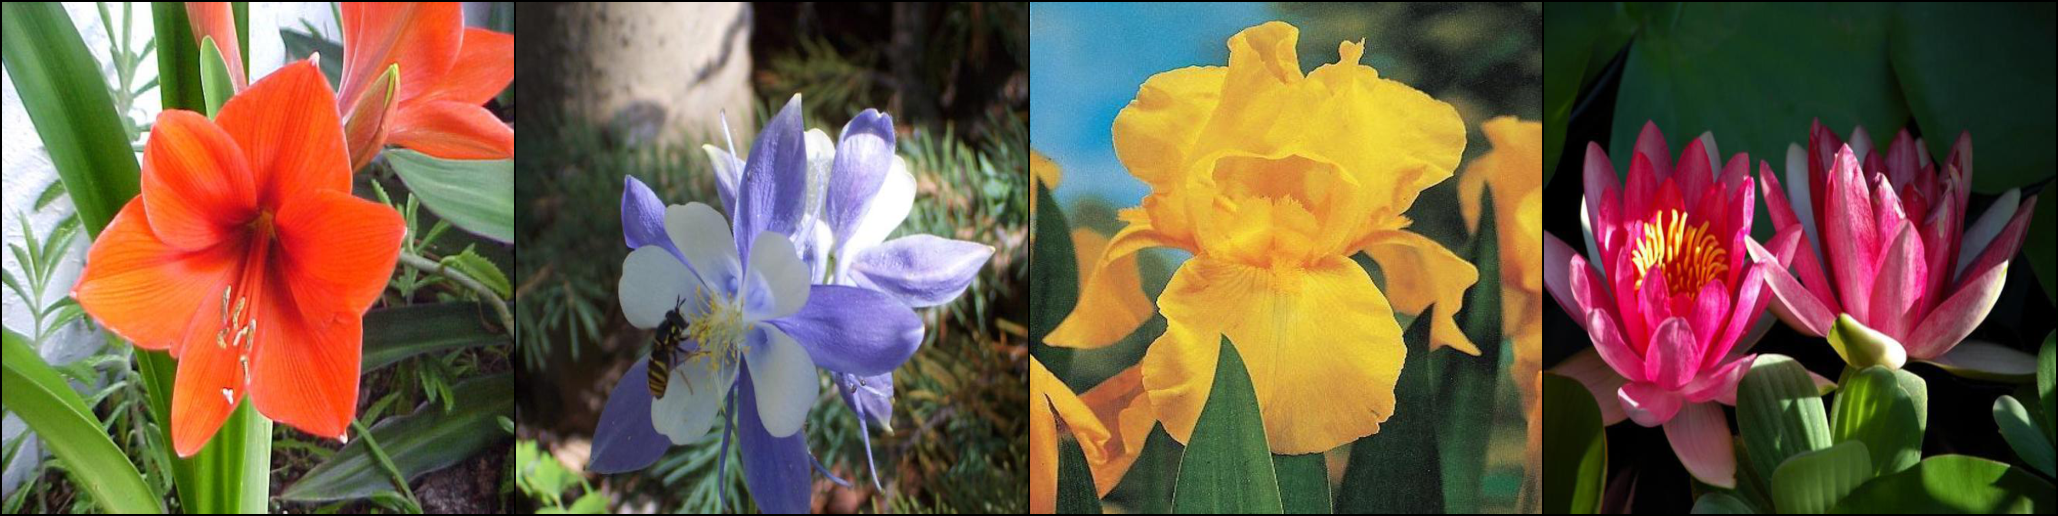
\includegraphics[width=\textwidth]{images/real_samples}
        \caption{Small excerpt from the \textit{102 Category Flower} dataset. The flowers offer a rich variety of colors, which perfectly fit for the visualization of music.}
        \label{flowers}
    \end{figure}